\section{Results}

This chapter reports the outcomes of the six mechanism-level experiments described in Chapter 4, one subsection per experiment, in the order E1, E2, E3, E4, G1, G2. Every figure, table, and number below is drawn directly from the committed CSVs under \texttt{experiments/results/} and the six figures under \texttt{experiments/analysis/figures/}. The chapter reports what was measured. It does not interpret those measurements against the architecture's design goals or SIDS 2026's open questions, which is the task of Chapter 6.

\subsection{E1: Signature-Verification Cost at the Edge}


\begin{figure}[H]
\centering
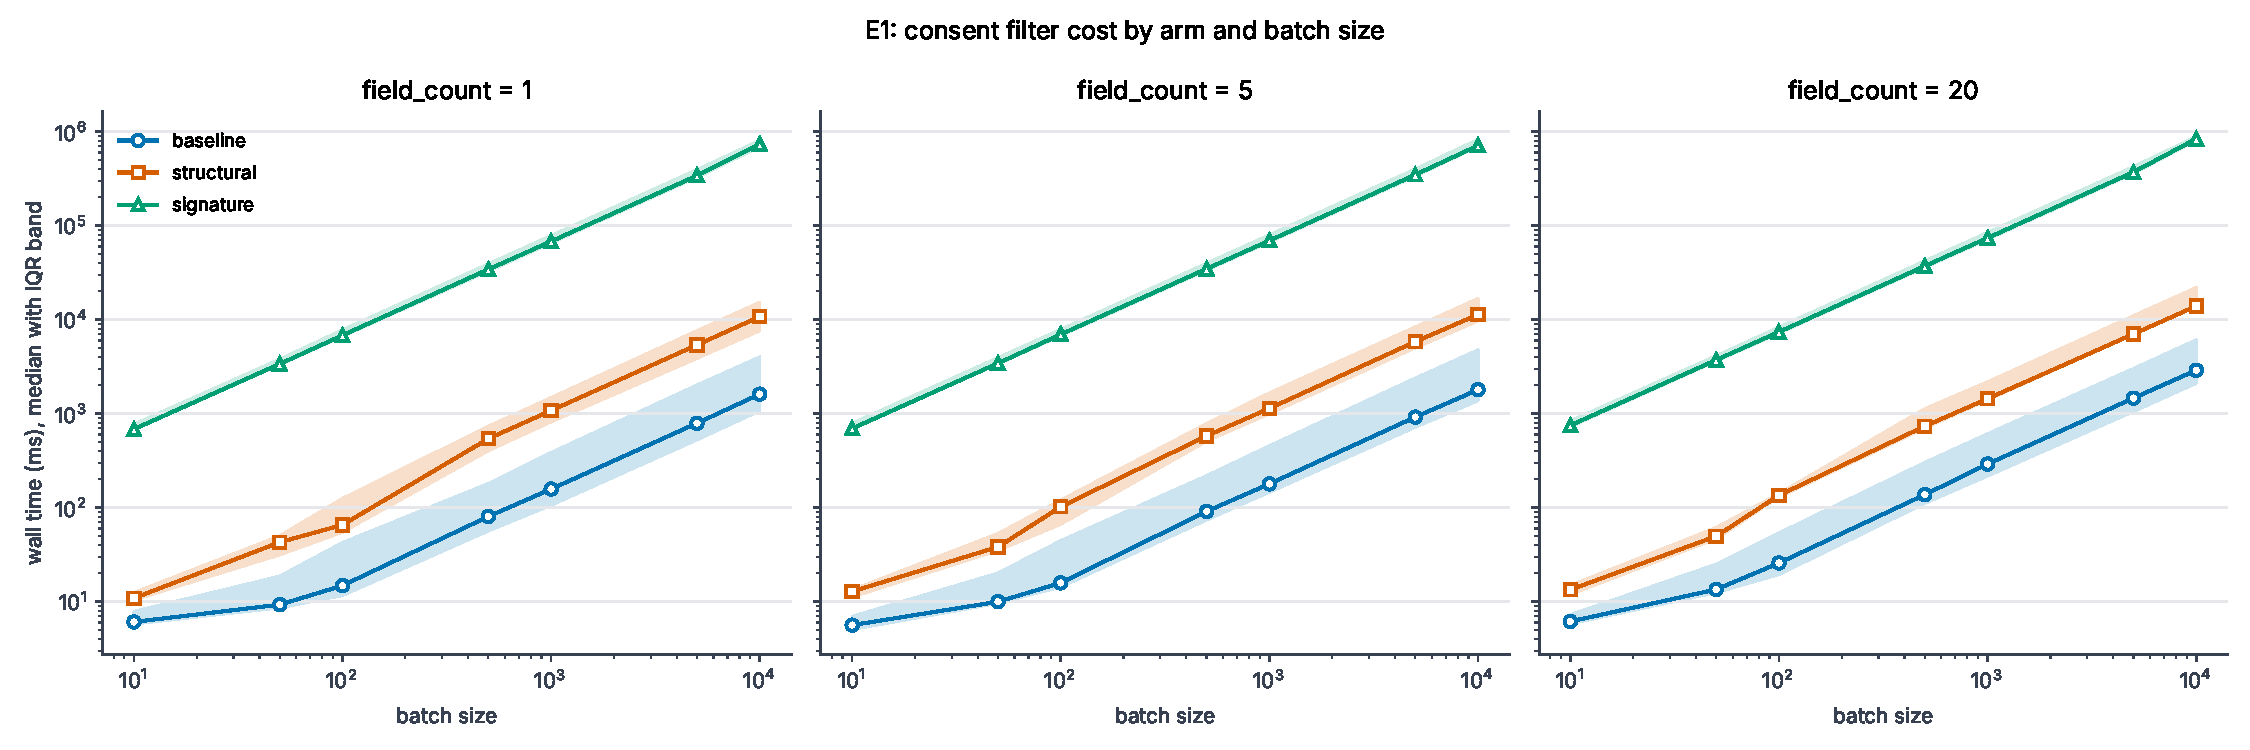
\includegraphics[width=0.9\linewidth]{../../experiments/analysis/figures/e1-crossover.pdf}
\caption{E1: signature-verification cost at the edge. Median wall time against batch size for the baseline, structural, and signature arms on log-log axes, one panel per field count (1, 5, 20). IQR bands shown for each arm.}
\end{figure}

Figure 1 (e1-crossover.pdf) plots median wall time against batch size for the three arms, baseline, structural, and signature, on log-log axes, one panel per field count. Across all three panels and the full swept batch-size range, from the smallest batch of 10 documents to the largest of 10,000, the three arms hold a fixed vertical ordering with no crossing: signature is costliest, structural is intermediate, and baseline is cheapest, at every plotted point.

At field\_count = 1 and the smallest swept batch (10 documents), median wall time is 6.07 ms (IQR 2.09 ms) for baseline, 10.85 ms (IQR 2.07 ms) for structural, and 682.41 ms (IQR 97.02 ms) for signature, a gap already present at the smallest batch the sweep tested: signature verification costs roughly 63 times the structural arm and 112 times the baseline arm at this point. The gap does not narrow as batch size grows. At the same field count and the largest swept batch (10,000 documents), median wall time is 1,607.78 ms (IQR 2,938.21 ms) for baseline, 10,735.27 ms (IQR 7,651.16 ms) for structural, and 731,749.77 ms (IQR 117,291.37 ms) for signature, a ratio of roughly 68 times structural and 455 times baseline. Across all three field counts and all seven batch sizes, the signature-to-structural ratio stays within a 50-to-104-fold band and the signature-to-baseline ratio within a 112-to-460-fold band. Neither ratio trends toward parity at any point in the swept range. At field\_count = 20, the largest field count tested, the pattern holds identically: signature median time runs from 748.32 ms at batch size 10 to 836,537.02 ms at batch size 10,000, remaining the costliest arm throughout. Table 3 gives the full field\_count = 1 sweep behind the two endpoints just quoted.

\begin{table}[H]
\caption{E1 wall time by batch size and arm, field\_count = 1, median (IQR) in milliseconds.\label{tab:t3}}
\small
\begin{tabular}{rrrr}
\toprule
Batch size & Baseline (ms) & Structural (ms) & Signature (ms) \\
\midrule
10 & 6.07 (IQR 2.09) & 10.85 (IQR 2.07) & 682.41 (IQR 97.02) \\
50 & 9.27 (IQR 10.05) & 42.75 (IQR 18.58) & 3,370.29 (IQR 478.45) \\
100 & 14.78 (IQR 30.81) & 65.38 (IQR 70.45) & 6,799.43 (IQR 1,147.54) \\
500 & 80.34 (IQR 123.86) & 540.02 (IQR 329.87) & 34,191.66 (IQR 6,511.47) \\
1,000 & 157.25 (IQR 278.55) & 1,076.41 (IQR 662.53) & 67,888.55 (IQR 13,159.07) \\
5,000 & 789.80 (IQR 1,487.63) & 5,372.79 (IQR 3,741.41) & 339,802.61 (IQR 66,529.45) \\
10,000 & 1,607.78 (IQR 2,938.21) & 10,735.27 (IQR 7,651.16) & 731,749.77 (IQR 117,291.37) \\
\bottomrule
\end{tabular}
\end{table}

There is no crossover point anywhere in the data. Signature verification is the dominant cost from the smallest batch onward, not a cost that overtakes the other arms past some threshold batch size. The three lines in Figure 1 run parallel on the log-log plot rather than intersecting.

The signature arm exists only inside E1's harness: it runs against a separate CouchDB design document (\texttt{build-signature-design-doc.ts}) that E1 builds and installs itself, never against the production \texttt{consent-couchdb} design document any real deployment's provisioning path installs. The production S1 filter performs no per-record signature verification of any kind. The three arms above measure what per-record signature verification would cost if it were added to the write path, not a cost the deployed system currently pays.

\subsection{E2: Revocation Propagation Under Network Partition}


\begin{figure}[H]
\centering
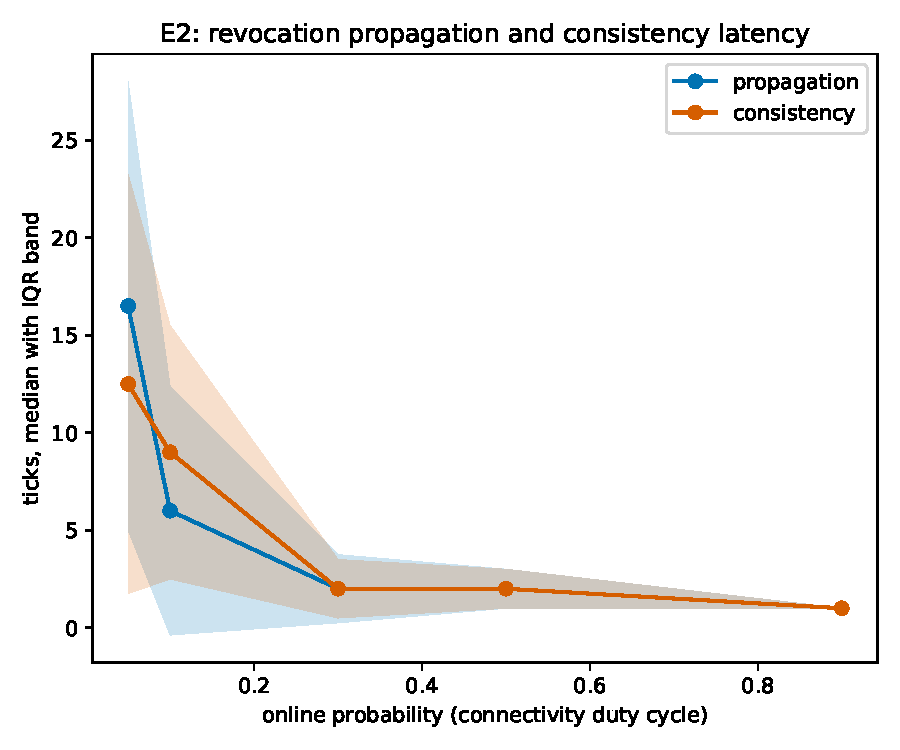
\includegraphics[width=0.9\linewidth]{../../experiments/analysis/figures/e2-propagation.pdf}
\caption{E2: revocation propagation and consistency latency against online probability, with IQR bands.}
\end{figure}

Figure 2 (e2-propagation.pdf) plots median propagation ticks and median consistency ticks against online probability, the duty-cycle parameter governing how often a simulated device comes online, swept across five values: 0.05, 0.1, 0.3, 0.5, and 0.9. Both curves fall sharply at low connectivity and flatten as connectivity increases. Median propagation ticks are 16.5 at online\_probability = 0.05, 6.0 at 0.1, 2.0 at 0.3, 2.0 at 0.5, and 1.0 at 0.9. Median consistency ticks follow a similar shape: 12.5 at 0.05, 9.0 at 0.1, 2.0 at 0.3, 2.0 at 0.5, and 1.0 at 0.9. Both series converge to the same value, 2.0 ticks, at online\_probability = 0.3 and 0.5, and both reach a floor of 1.0 tick at the highest tested connectivity, online\_probability = 0.9. The IQR bands are widest at the lowest connectivity value (propagation IQR of 23 ticks and consistency IQR of 21.5 ticks at online\_probability = 0.05) and narrow to zero by online\_probability = 0.9, reflecting the point at which nearly every device is online on nearly every tick. Table 4 gives the full sweep.

\begin{table}[H]
\caption{E2 propagation and consistency ticks by online probability, median (IQR).\label{tab:t4}}
\small
\begin{tabular}{rrrrr}
\toprule
Online probability & Prop. Median (ticks) & Prop. IQR & Cons. Median (ticks) & Cons. IQR \\
\midrule
0.05 & 16.5 & 23 & 12.5 & 21.5 \\
0.1 & 6 & 12.75 & 9 & 13 \\
0.3 & 2 & 3.5 & 2 & 3 \\
0.5 & 2 & 2 & 2 & 2 \\
0.9 & 1 & 0 & 1 & 0 \\
\bottomrule
\end{tabular}
\end{table}

Across all five sweep points, pooling 90 data points per point for both the revocation-device and conflict-device measurements (150 independent fleet trials in total, 30 per sweep point), the leaked-record count and the unresolved-conflict count are both 0. No trial, at any tested connectivity level including the most disconnected duty cycle tested (online\_probability = 0.05), produced a record visible in the shared CouchDB database for a purpose the owning participant had revoked, and no trial left an injected conflict unresolved by the end of its run.

\subsection{E3: Audit-Chain Verification Cost at Scale}


\begin{figure}[H]
\centering
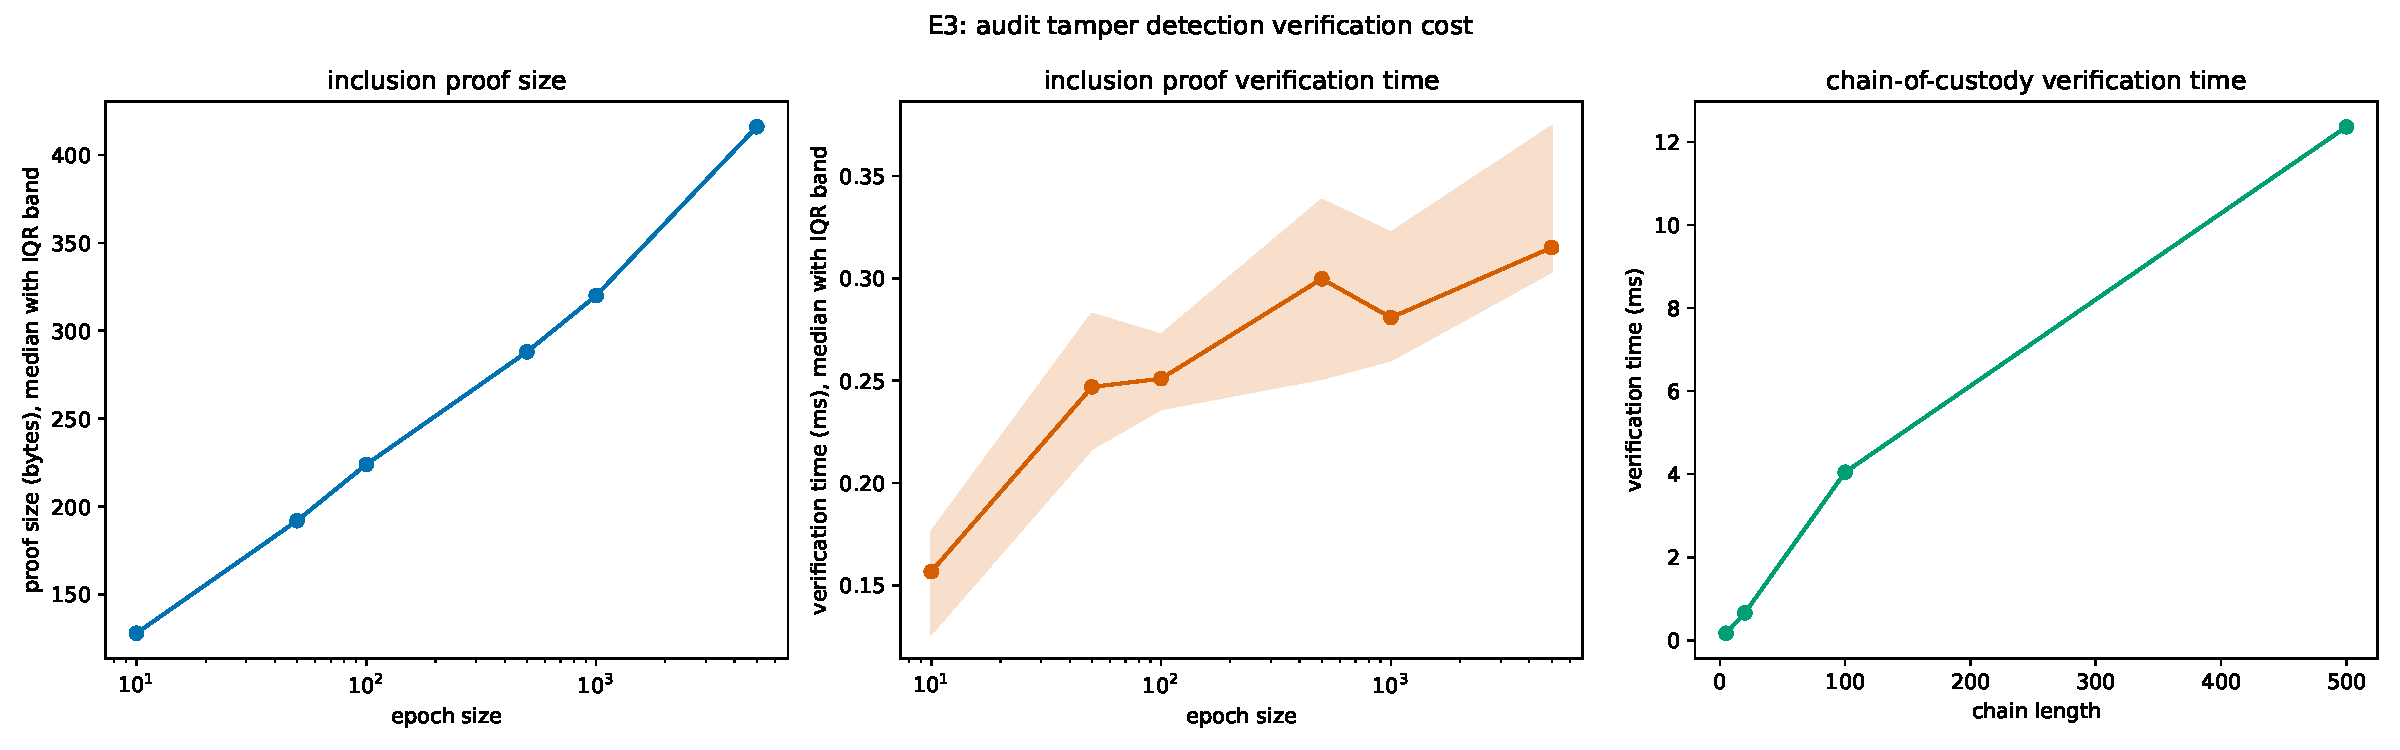
\includegraphics[width=0.9\linewidth]{../../experiments/analysis/figures/e3-verification-cost.pdf}
\caption{E3: audit-chain verification cost at scale. (\textbf{a}) Inclusion proof size against epoch size. (\textbf{b}) Inclusion-proof verification time against epoch size. (\textbf{c}) Chain-of-custody verification time against chain length.}
\end{figure}

Figure 3 (e3-verification-cost.pdf) presents three panels: inclusion proof size and inclusion-proof verification time, both swept against epoch size on a log x-axis, and chain-of-custody verification time swept against chain length.

Median proof size grows from 128 bytes at epoch\_size = 10 to 416 bytes at epoch\_size = 5000, passing through 192 bytes at epoch\_size = 50, 224 bytes at epoch\_size = 100, 288 bytes at epoch\_size = 500, and 320 bytes at epoch\_size = 1000. Median inclusion-proof verification time rises over the same sweep from 0.157 ms at epoch\_size = 10 to 0.315 ms at epoch\_size = 5000, with intermediate medians of 0.247 ms at epoch\_size = 50, 0.251 ms at epoch\_size = 100, 0.300 ms at epoch\_size = 500, and a slight dip to 0.281 ms at epoch\_size = 1000 before rising again at the largest epoch size. Every inclusion-proof verification measured across the full sweep stays under one millisecond. Chain-of-custody verification time, measured separately against chain length rather than epoch size since it depends only on the number of epochs to compare and not their internal size, rises from 0.169 ms at a chain length of 5 to 12.364 ms at a chain length of 500, passing through 0.660 ms at chain length 20 and 4.047 ms at chain length 100, each point the median of ten timed repetitions following an untimed warmup pass, the same protocol section 4.3 describes. Table 5 gives the epoch-size sweep and Table 6 the chain-length sweep behind these numbers.

\begin{table}[H]
\caption{E3 inclusion-proof size and verification time by epoch size, median (IQR).\label{tab:t5}}
\begin{tabularx}{\textwidth}{rrX}
\toprule
Epoch size & Proof size, median (bytes) & Inclusion verification, median ms (IQR) \\
\midrule
10 & 128 & 0.157 (IQR 0.049) \\
50 & 192 & 0.247 (IQR 0.065) \\
100 & 224 & 0.251 (IQR 0.036) \\
500 & 288 & 0.300 (IQR 0.087) \\
1,000 & 320 & 0.281 (IQR 0.062) \\
5,000 & 416 & 0.315 (IQR 0.071) \\
\bottomrule
\end{tabularx}
\end{table}

\begin{table}[H]
\caption{E3 chain-of-custody verification time by chain length, median of ten timed repetitions.\label{tab:t6}}
\small
\begin{tabular}{rr}
\toprule
Chain length & Verification time, median (ms) \\
\midrule
5 & 0.169 \\
20 & 0.660 \\
100 & 4.047 \\
500 & 12.364 \\
\bottomrule
\end{tabular}
\end{table}

Tamper detection itself is not a quantity this sweep measures. E3's harness times and sizes calls into audit-chain logic that an earlier implementation phase already tested at the boolean level, and it deliberately performs no tamper injection of its own. That earlier phase's own test suite (\texttt{MerkleTreeTest.java} and \texttt{packages/audit-verify}'s \texttt{chain.test.ts}) establishes 100\% tamper detection at the mechanism level: a wrong leaf, a mutated root, and a tampered proof step each fail inclusion verification, and a reordered or mutated-root epoch is caught by chain verification, in every case tested. E3's contribution is the cost curve layered on top of that already-established correctness result, not a re-measurement of detection accuracy itself.

\subsection{E4: Privacy-Budget-Versus-Utility Tradeoff}


\begin{figure}[H]
\centering
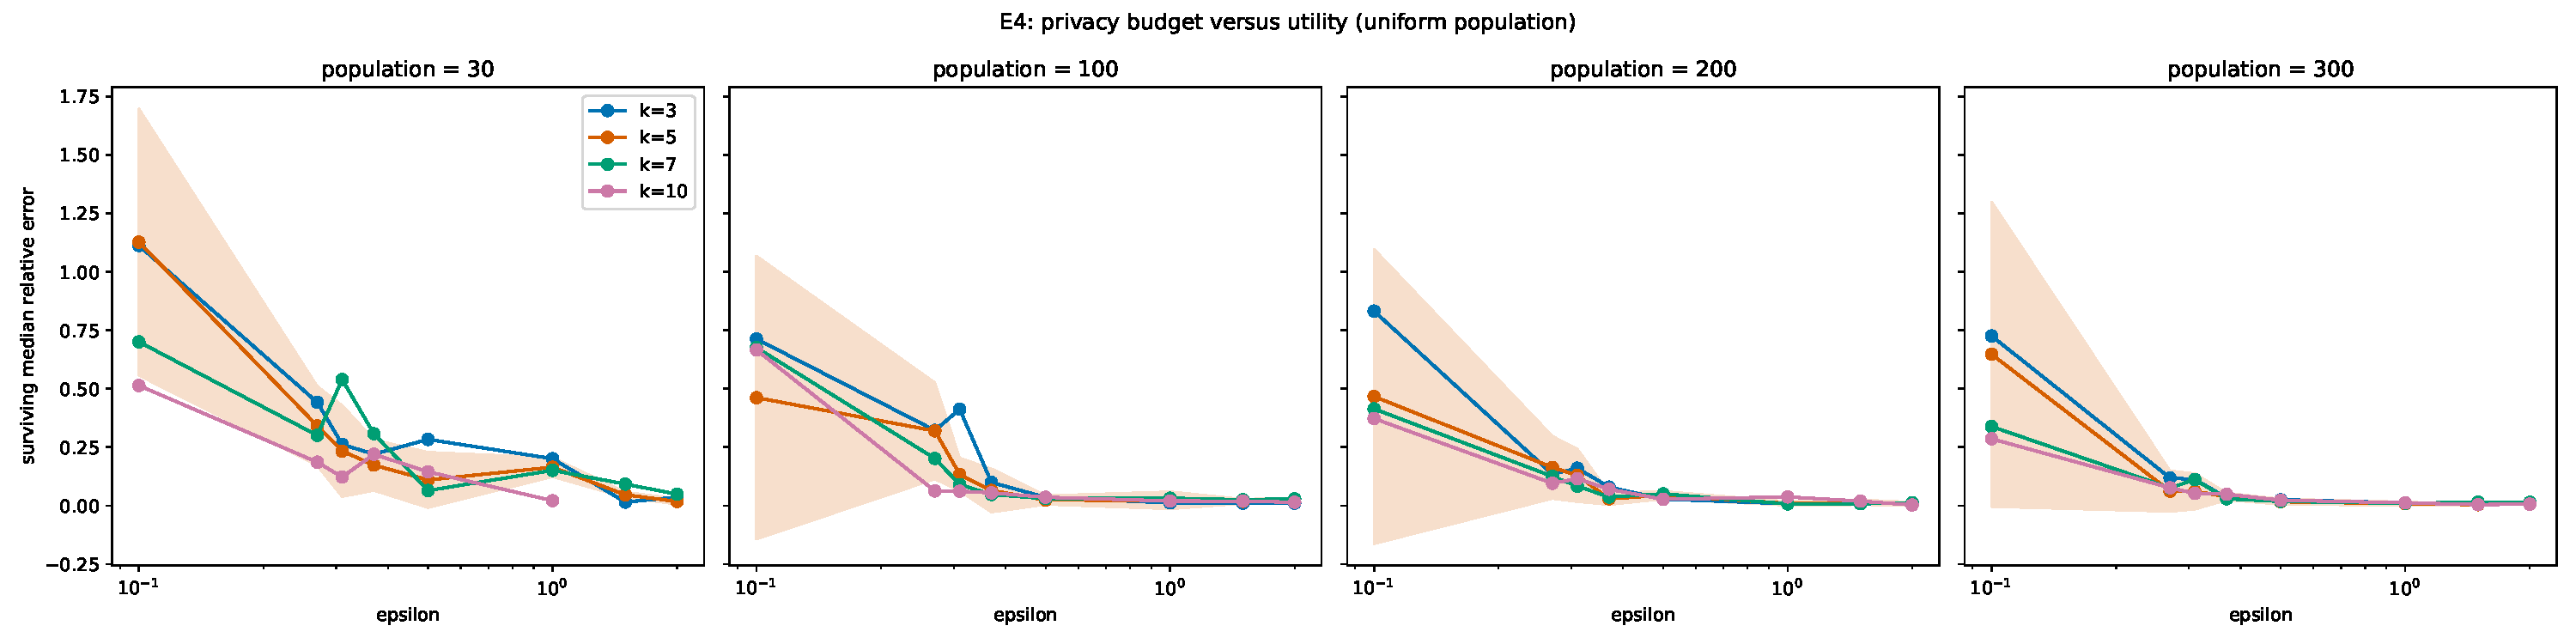
\includegraphics[width=0.9\linewidth]{../../experiments/analysis/figures/e4-utility.pdf}
\caption{E4: privacy-budget-versus-utility tradeoff. Surviving median relative error against epsilon, one panel per population size, one line per k threshold, uniform skew only.}
\end{figure}

Figure 4 (e4-utility.pdf) plots the surviving median relative error, computed only over query results that were neither k-anonymity suppressed nor budget refused, against epsilon on a log x-axis, one panel per population size (30, 100, 200, 300), one line per k threshold (3, 5, 7, 10), restricted to the uniform population-skew slice of the swept grid. The surviving-only statistic is used deliberately: the plain median-relative-error column is pinned at a sentinel value of 1.0 across nearly the entire swept grid, since it assigns that sentinel to every suppressed or refused group rather than reporting the accuracy of the answers that were actually returned, and would show a flat, uninformative line rather than the real accuracy-versus-epsilon relationship.

The dominant pattern across all four population panels is that surviving median relative error falls as epsilon rises, most steeply between epsilon = 0.1 and epsilon = 0.5, then flattening toward a low floor by epsilon = 1.0 and above. At population = 30, the smallest tested, surviving median relative error at epsilon = 0.1 ranges from 0.513 (k = 10, IQR 0.502) to 1.127 (k = 5, IQR 1.140) across the four k values, and falls to a range of 0.017 to 0.049 by epsilon = 2.0, though at that same population and epsilon the surviving-point counts are again thin, 5, 3, 3, and 0 of 68 across the four k values (k = 10 has no surviving points at all at this cell), so this epsilon = 2.0 accuracy floor carries the same thin-sample caveat as the epsilon = 0.1 figures below. At population = 300, the largest tested, the same statistic starts lower at epsilon = 0.1, ranging from 0.286 (k = 10, IQR 0.579) to 0.726 (k = 3, IQR 1.223), and falls to a range of 0.006 to 0.014 by epsilon = 2.0. Suppression is heaviest at the combination of small population and high k: at population = 30, k = 10, the suppression/refusal rate is 95.6\% at epsilon = 0.1 and reaches 100\% at epsilon = 1.5 and epsilon = 2.0, meaning zero surviving data points at those two grid cells and no surviving-error value to report there. At population = 300, suppression is markedly lighter at low epsilon: the suppression/refusal rate at epsilon = 0.1 ranges from 6.5\% (k = 3) to 56.1\% (k = 10), compared with 64.7\% to 95.6\% at population = 30 for the same k values. Table 7 gives these two population panels' endpoint epsilon values side by side, with the surviving-point count behind each figure.

\begin{table}[H]
\caption{E4 surviving median relative error at epsilon = 0.1 and epsilon = 2.0, uniform skew, median (IQR) [surviving points / total grid points].\label{tab:t7}}
\small
\begin{tabular}{rrrr}
\toprule
Population & k & epsilon = 0.1 & epsilon = 2.0 \\
\midrule
30 & 3 & 1.113 (IQR 1.798) [n=24/68] & 0.036 (IQR 0.087) [n=5/68] \\
30 & 5 & 1.127 (IQR 1.140) [n=13/68] & 0.017 (IQR 0.023) [n=3/68] \\
30 & 7 & 0.701 (IQR 0.383) [n=10/68] & 0.049 (IQR 0.070) [n=3/68] \\
30 & 10 & 0.514 (IQR 0.502) [n=3/68] & no surviving points [n=0/68] \\
300 & 3 & 0.726 (IQR 1.223) [n=100/107] & 0.008 (IQR 0.007) [n=5/107] \\
300 & 5 & 0.647 (IQR 1.304) [n=86/107] & 0.009 (IQR 0.009) [n=5/107] \\
300 & 7 & 0.338 (IQR 0.860) [n=62/107] & 0.014 (IQR 0.015) [n=5/107] \\
300 & 10 & 0.286 (IQR 0.579) [n=47/107] & 0.006 (IQR 0.004) [n=5/107] \\
\bottomrule
\end{tabular}
\end{table}

The population = 30, epsilon = 0.1 numbers just reported carry sharply unequal statistical weight across k, since the surviving-only statistic is computed only over the queries that were not suppressed or refused at that cell: the 0.513 figure for k = 10 is a median over 3 surviving data points out of 68, the k = 7 figure over 10, the k = 5 figure over 13, and the k = 3 figure over 24. A reader comparing 0.513 (k = 10) against 1.127 (k = 5) at this cell is comparing a statistic computed on 3 points against one computed on 13, not two equally-supported estimates, and the k = 10 figure in particular should be read as illustrative of the few queries that happened to clear suppression at that combination rather than as a stable estimate of typical accuracy there. The same caution applies wherever a low-epsilon, small-population, high-k cell is quoted elsewhere in this section or in Chapter 6.

\subsection{G1: Quorum Availability Under the Built Policy and the Veto Policy SIDS 2026 Specified}


\begin{figure}[H]
\centering
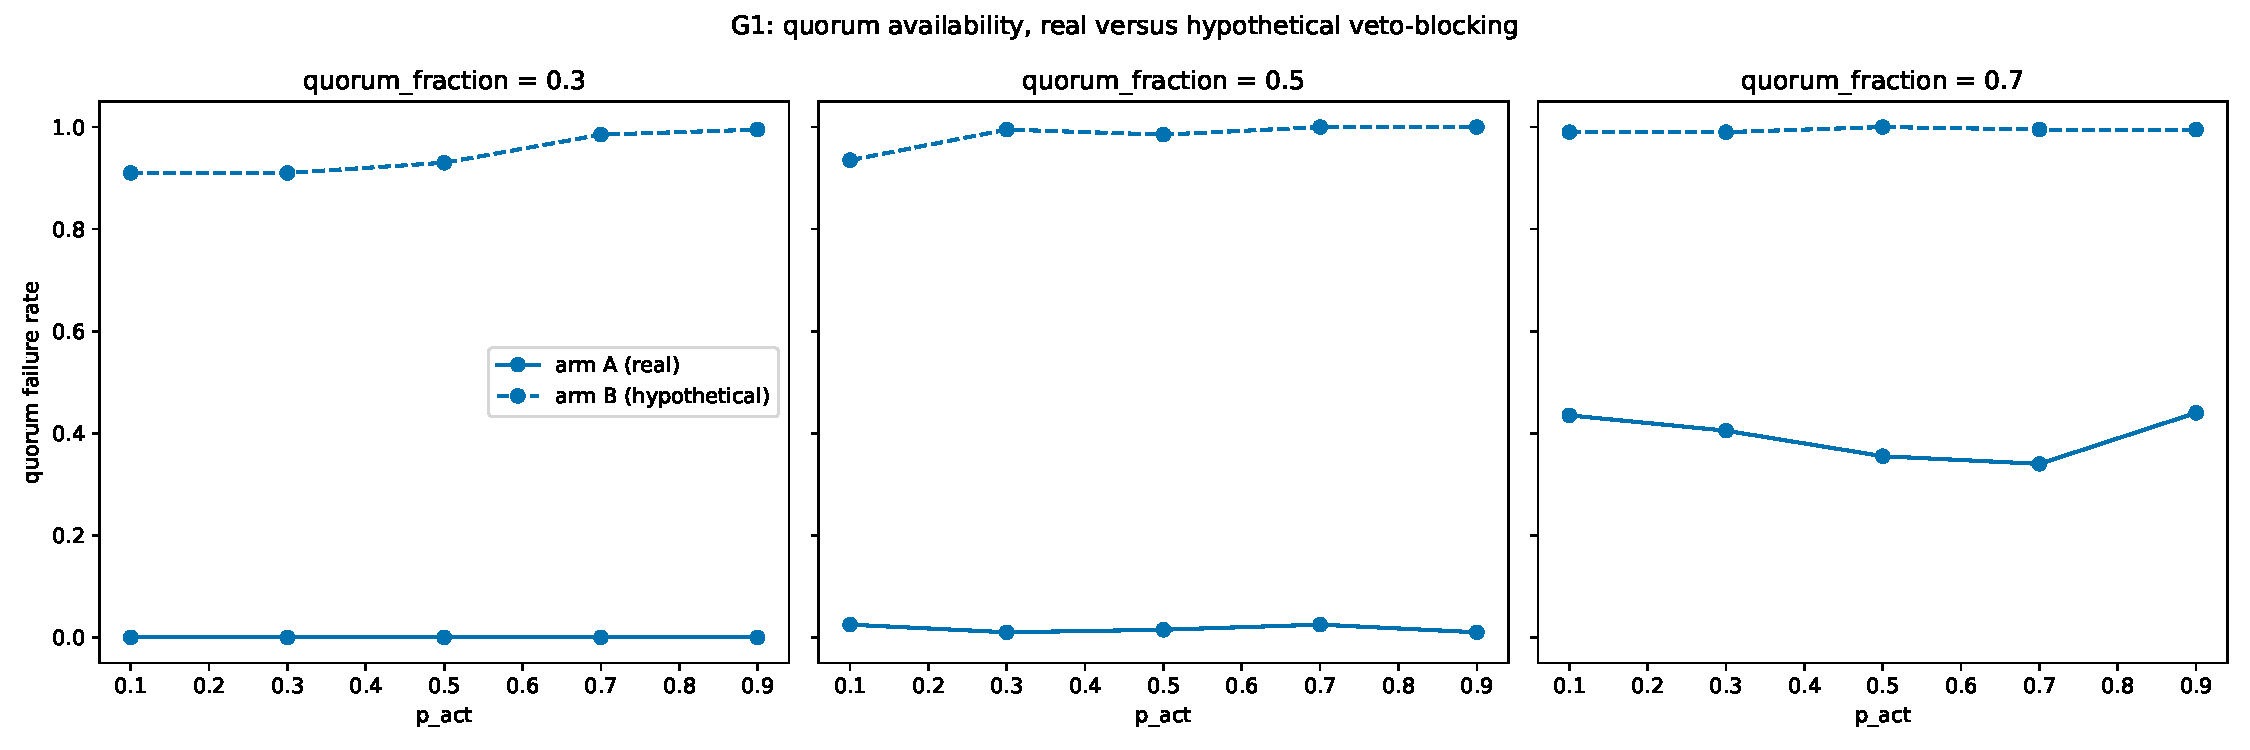
\includegraphics[width=0.9\linewidth]{../../experiments/analysis/figures/g1-availability.pdf}
\caption{G1: quorum failure rate against action probability for Arm A (the built, veto-blind policy) and Arm B (SIDS 2026's specified veto policy), one panel per quorum fraction.}
\end{figure}

Figure 5 (g1-availability.pdf) plots quorum failure rate against per-tick action probability (p\_act), one panel per quorum fraction (0.3, 0.5, 0.7), comparing two lines. Arm A drives the real, unmodified \texttt{StewardQuorumFunction}, the built system's policy: a release clears once the same swept quorum count Q has signed, and a recorded veto has no effect on that decision, matching section 3.4's disclosure. Arm B drives a second decision function that adds exactly the check SIDS 2026 specified and the built system omits: the identical swept quorum count Q as Arm A (SIDS 2026's own text names two-of-three co-signature as the specific case of this rule), plus a permanent block the moment any single steward vetoes, evaluated on the identical simulated timeline as Arm A so the only difference between the two lines is whether the veto SIDS 2026 promised is actually enforced. Arm A's failure rate is computed as 1 minus its reached rate. Arm B's is computed as its starved rate plus its vetoed rate, since Arm B's failures split across two mutually exclusive outcomes and its starved rate alone would omit its dominant failure mode. Both arms are shown at the filtered slice veto\_share = 0.3 and N = 20, the largest tested veto share and the largest tested steward pool, the combination that shows the clearest separation between the two policies. This slice yields 15 plotted points, five p\_act values across each of three quorum-fraction panels.

Framed this way, G1 does not compare the built system against an arbitrary stricter alternative. It measures the availability cost of enforcing the veto guarantee SIDS 2026 actually specified in its own text, a guarantee the implementation currently does not provide. Arm A fails far less often than Arm B at every one of the 15 plotted points, precisely because Arm A never lets a veto stop a release. At quorum\_fraction = 0.3, Arm A's failure rate is 0.0 across all five tested p\_act values (median ticks-to-quorum 1.0 to 6.0, IQR 0.0 to 3.0), while Arm B's failure rate ranges from 0.910 (p\_act = 0.1 and 0.3) to 0.995 (p\_act = 0.9). At quorum\_fraction = 0.5, Arm A's failure rate ranges from 0.010 to 0.025 (median ticks-to-quorum 1.0 to 12.0, IQR up to 7.0 at p\_act = 0.1), while Arm B's ranges from 0.935 to 1.0. At quorum\_fraction = 0.7, the panel with the narrowest gap, Arm A's failure rate ranges from 0.340 to 0.440 (median ticks-to-quorum 1.0 to 20.0, IQR up to 10.0 at p\_act = 0.1), while Arm B's ranges from 0.990 to 1.0. Table 8 gives all 15 plotted points, splitting each arm's failure rate into its component causes.

\begin{table}[H]
\caption{G1 quorum failure rate and its components, veto\_share = 0.3, N = 20.\label{tab:t8}}
\small
\begin{tabular}{rrrrrrr}
\toprule
Quorum frac. & p\_act & A fail rate & A starved rate & B fail rate & B vetoed rate & B starved rate \\
\midrule
0.3 & 0.1 & 0.000 & 0.000 & 0.910 & 0.910 & 0.000 \\
0.3 & 0.3 & 0.000 & 0.000 & 0.910 & 0.910 & 0.000 \\
0.3 & 0.5 & 0.000 & 0.000 & 0.930 & 0.930 & 0.000 \\
0.3 & 0.7 & 0.000 & 0.000 & 0.985 & 0.985 & 0.000 \\
0.3 & 0.9 & 0.000 & 0.000 & 0.995 & 0.995 & 0.000 \\
0.5 & 0.1 & 0.025 & 0.025 & 0.935 & 0.935 & 0.000 \\
0.5 & 0.3 & 0.010 & 0.010 & 0.995 & 0.995 & 0.000 \\
0.5 & 0.5 & 0.015 & 0.015 & 0.985 & 0.985 & 0.000 \\
0.5 & 0.7 & 0.025 & 0.025 & 1.000 & 1.000 & 0.000 \\
0.5 & 0.9 & 0.010 & 0.010 & 1.000 & 1.000 & 0.000 \\
0.7 & 0.1 & 0.435 & 0.435 & 0.990 & 0.990 & 0.000 \\
0.7 & 0.3 & 0.405 & 0.405 & 0.990 & 0.990 & 0.000 \\
0.7 & 0.5 & 0.355 & 0.355 & 1.000 & 1.000 & 0.000 \\
0.7 & 0.7 & 0.340 & 0.340 & 0.995 & 0.995 & 0.000 \\
0.7 & 0.9 & 0.440 & 0.440 & 0.995 & 0.995 & 0.000 \\
\bottomrule
\end{tabular}
\end{table}

Computed pointwise across all 15 plotted points, the divergence between Arm B's failure rate and Arm A's failure rate has a minimum of 0.555, occurring at quorum\_fraction = 0.7, and a maximum of 0.995, occurring at quorum\_fraction = 0.3, p\_act = 0.9. At no plotted point does the gap between the two arms fall below 0.555: enforcing the veto SIDS 2026 specified would raise the quorum failure rate far above what the built, veto-blind policy currently exhibits at every combination of quorum fraction and action probability tested.

Splitting Arm B's failure rate into its two mutually exclusive components at this same slice shows that the gap is driven almost entirely by vetoes rather than by genuine starvation. At all 15 plotted points, \texttt{arm\_b\_starved\_rate} is 0.0: no run in this slice reaches \texttt{maxTicks} without either quorum or a veto. \texttt{arm\_b\_vetoed\_rate} alone accounts for the entire failure rate reported above, from 0.910 at quorum\_fraction = 0.3, p\_act = 0.1, to 1.0 at several points in the quorum\_fraction = 0.5 and 0.7 panels (for example quorum\_fraction = 0.5, p\_act = 0.7 and 0.9, and quorum\_fraction = 0.7, p\_act = 0.5). This means Arm B's high failure rate is not evidence that the veto-enforcing policy is prone to stalling independently of stewards' objections. It is a direct, mechanical consequence of a 0.3 veto share applied across a pool of 20 stewards, where enough stewards act that at least one veto lands before quorum is reached almost every time. The veto mechanism, when actually enforced, works as specified: it blocks release whenever a steward objects. What the data show is the availability price of that guarantee at this veto share, not a separate defect in the quorum-reaching logic itself. Arm A, by contrast, does exhibit genuine starvation at the higher quorum fractions independent of any veto, since it ignores vetoes entirely: \texttt{arm\_a\_starved\_rate} reaches 0.435 at quorum\_fraction = 0.7, p\_act = 0.1, reflecting only that not enough stewards signed within the 200-tick horizon, the one failure mode Arm A can have.

\subsection{G2: Consent Heterogeneity Versus Aggregate Utility}


\begin{figure}[H]
\centering
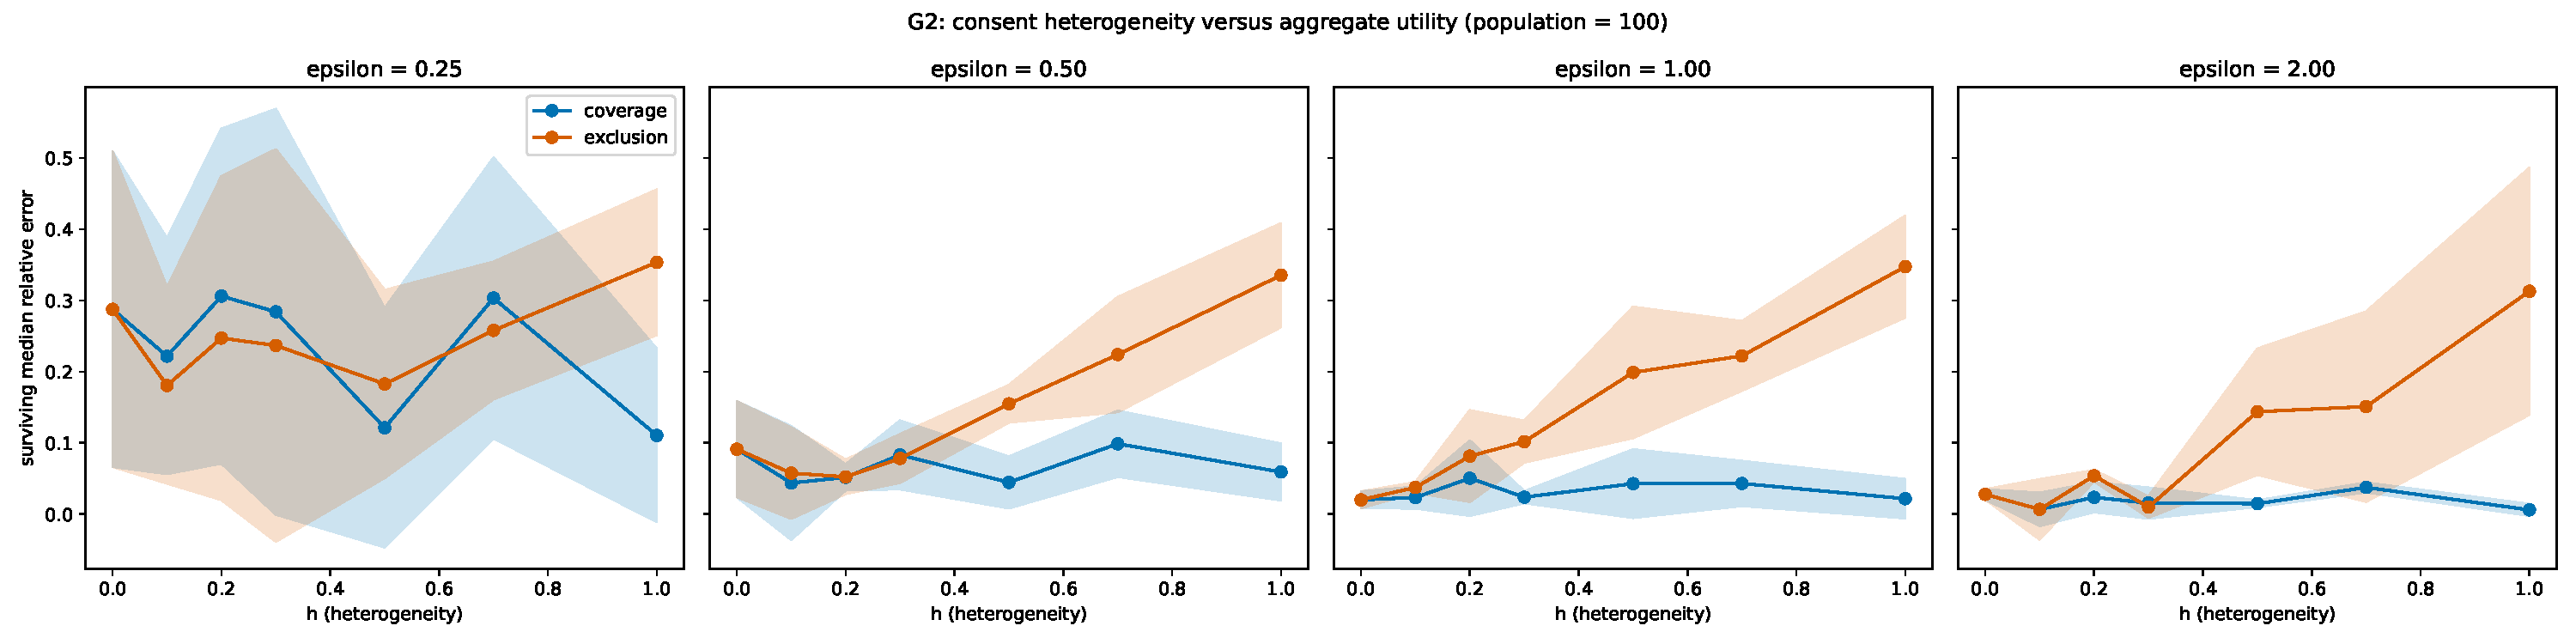
\includegraphics[width=0.9\linewidth]{../../experiments/analysis/figures/g2-heterogeneity.pdf}
\caption{G2: surviving coverage error and surviving exclusion error against consent heterogeneity h, one panel per epsilon, with IQR bands.}
\end{figure}

Figure 6 (g2-heterogeneity.pdf) plots two surviving-only relative-error statistics against heterogeneity h, one panel per epsilon (0.25, 0.5, 1.0, 2.0), restricted to population = 100. Both statistics are computed from the same noised \texttt{PrivacyPipeline.compute()} output. They differ only in which ground truth that noised output is compared against. Surviving coverage error compares the observed, noised result against the consenting population's own true count, so the consenting population is already the reference: this statistic isolates the DP mechanism's own noise, since the population it is measured against has already had heterogeneous consent's exclusions applied to it before the comparison is made. Surviving exclusion error compares the same observed, noised result against the full generated population's true count, unfiltered by consent: this statistic captures total distortion against the true community value, noise and exclusion bias together, not exclusion bias in isolation and not a quantity computed before noise is applied. It is the gap between exclusion error and coverage error, not exclusion error alone, that isolates the effect of heterogeneous consent specifically, since that gap is exactly the part of the total distortion coverage error's noise-only comparison does not already account for. As with E4, the surviving-only columns are used because the plain coverage- and exclusion-error columns are pinned at a sentinel value across most of the swept grid.

At epsilon = 1.0, surviving exclusion error rises from 0.020 (IQR 0.023) at h = 0.0 to 0.348 (IQR 0.142) at h = 1.0, passing through 0.037 at h = 0.1, 0.081 at h = 0.2, 0.102 at h = 0.3, 0.199 at h = 0.5, and 0.222 at h = 0.7, a roughly seventeen-fold increase across the heterogeneity sweep. At epsilon = 2.0, exclusion error also ends far above where it starts, rising from 0.028 at h = 0.0 to 0.313 at h = 1.0, though the path between those endpoints is not strictly monotonic: it dips to 0.007 at h = 0.1 and to 0.010 at h = 0.3 before climbing through 0.144 at h = 0.5 and 0.151 at h = 0.7 on the way to the h = 1.0 maximum. Surviving coverage error over the same two epsilon values shows no comparable overall trend: at epsilon = 1.0 it ranges narrowly from 0.020 (IQR 0.023) to 0.050 (IQR 0.105 at h = 0.2) across the full h sweep with no monotonic direction, and at epsilon = 2.0 it ranges from 0.006 to 0.037, again without trending upward as h increases. At the lowest tested epsilon (0.25), where Laplace noise is largest, both statistics are noisier and the separation is less clean, coverage error ranges from 0.111 to 0.306 (IQR from 0.243 to 0.569 across the sweep) and exclusion error from 0.181 to 0.354 (IQR from 0.193 to 0.550), but exclusion error still reaches its sweep maximum at h = 1.0 (0.354) while coverage error does not show the same endpoint behavior (0.111 at h = 1.0, within the range seen at smaller h values). Because coverage error stays flat while exclusion error climbs, the gap between them, not exclusion error by itself, is the cleanest read of heterogeneity's own effect: at epsilon = 1.0 that gap widens from effectively 0.0 at h = 0.0 (where the two statistics are identical by construction) to roughly 0.326 at h = 1.0 (0.348 exclusion against 0.022 coverage), tracking the growth in excluded\_fraction reported below rather than any change in the noise mechanism itself. Read this way, G2's finding is more precise than "exclusion error grows with heterogeneity" alone: it is that heterogeneous consent introduces a distortion on top of DP noise, one that grows with h, while the DP mechanism's own noise contribution, measured by coverage error, does not. Table 9 gives the full h sweep at epsilon = 1.0 and epsilon = 2.0, alongside the excluded fraction reported below.

\begin{table}[H]
\caption{G2 surviving coverage and exclusion error by heterogeneity h, population = 100, median (IQR).\label{tab:t9}}
\small
\begin{tabular}{rrrrrr}
\toprule
h & Excl. Frac. & eps=1.0 cov. & eps=1.0 excl. & eps=2.0 cov. & eps=2.0 excl. \\
\midrule
0.0 & 0.00 & 0.020 (IQR 0.023) & 0.020 (IQR 0.023) & 0.028 (IQR 0.014) & 0.028 (IQR 0.014) \\
0.1 & 0.08 & 0.023 (IQR 0.030) & 0.037 (IQR 0.015) & 0.007 (IQR 0.046) & 0.007 (IQR 0.084) \\
0.2 & 0.16 & 0.050 (IQR 0.105) & 0.081 (IQR 0.128) & 0.024 (IQR 0.041) & 0.054 (IQR 0.015) \\
0.3 & 0.27 & 0.024 (IQR 0.016) & 0.102 (IQR 0.058) & 0.015 (IQR 0.043) & 0.010 (IQR 0.030) \\
0.5 & 0.49 & 0.043 (IQR 0.096) & 0.199 (IQR 0.184) & 0.015 (IQR 0.009) & 0.144 (IQR 0.177) \\
0.7 & 0.73 & 0.043 (IQR 0.063) & 0.222 (IQR 0.097) & 0.037 (IQR 0.013) & 0.151 (IQR 0.267) \\
1.0 & 1.00 & 0.022 (IQR 0.055) & 0.348 (IQR 0.142) & 0.006 (IQR 0.016) & 0.313 (IQR 0.346) \\
\bottomrule
\end{tabular}
\end{table}

The excluded fraction, the direct measurement of how much of the population lacked a valid grant for at least one query attribute, rises monotonically with h independent of epsilon: 0.0 at h = 0.0, 0.08 at h = 0.1, 0.16 at h = 0.2, 0.27 at h = 0.3, 0.49 at h = 0.5, 0.73 at h = 0.7, and 1.0 at h = 1.0.
